\section{1174008 - Arjun Yuda Firwanda}

\subsection{Teori}
\begin{enumerate}

        \item Kenapa file suara harus dilakukan MFCC
MFCC (Mel Frequency Cepstrum Coefficients) merupakan proses ekstraksi ciri dari sinyal wicara. Proses MFCC ini akan mengkonversikan sinyal suara menjadi beberapa vektor yang berguna untuk proses pengenalan. MFCC merupakan salah satu metode yang digunakan dalam bidang speech teknologi seperti speaaker recognition serta speech recognition. Selain itu juga spekearnya mampu Mampu untuk menangkap karakteristik suara yang sangat penting bagi pengenalan suara, serta dapat menangkap informasi-informasi penting yang terkandung dalam sinyal suara.

	\begin{figure}[H]
            	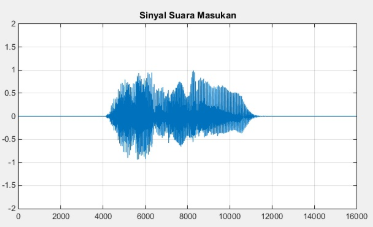
\includegraphics[width=3cm]{figures/1174008/6/teori1.PNG}
           	 \centering
           	 \caption{MFCC}
        	\end{figure}

        \item Konsep dasar Neural Network
Konsep dasar neural network sendiri di mulai dari ide dasar neural network dari otak manusia, dimana otak terdiri dari 1011 neuron. sehingga konsep dasar ini membangun neural network buatan yang disebut (Artificial Neural Network).

	\begin{figure}[H]
		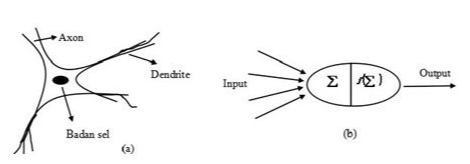
\includegraphics[width=3cm]{figures/1174008/6/teori2.PNG}
            	\centering
           	 \caption{Konsep Neural Network}
       	 \end{figure}

        \item Konsep Pembobotan dalam Neural Network
Konsep pembobotan dalam neural network sendiri menggunakan algoritma backpropagation untuk memperkecil tingkat eror dengan menyesuaikan nilai bobot berdasarkan perbedaan output serta target yang dicapai.

	\begin{figure}[H]
		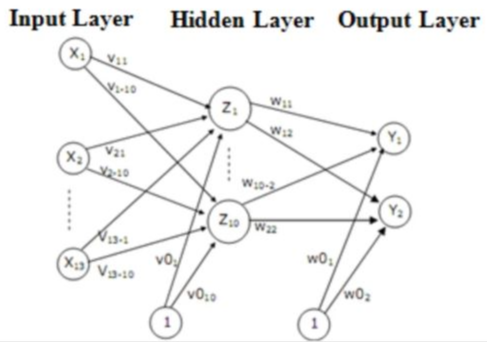
\includegraphics[width=3cm]{figures/1174008/6/teori3.PNG}
            	\centering
           	 \caption{Konsep Pembobotan Neural Network}
       	 \end{figure}

        \item Konsep Aktifasi dalam Neural Network
Fungsi aktivasi sendiri menggunakan nilai threshold untuk membatasi nilai keluaran agar selalu dalam batas nilai yang ditetapkan.

	\begin{figure}[H]
		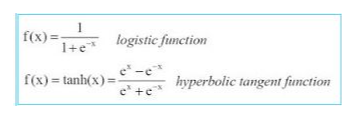
\includegraphics[width=3cm]{figures/1174008/6/teori4.PNG}
            	\centering
           	 \caption{Konsep Aktivasi Neural Network}
       	 \end{figure}

        \item cara membaca hasil PLOT dari MFCC
Cara membaca plot hasil mfcc dapat dilakukan dengan cara suara pengguna dijadikan file dalam bentuk *.wav yang digunakan sebagai inputan kemudian direpresentasikan menjadi sinyal suara dalam bentuk matriks dengan perintah auudiread di Matlab R2017a.

	\begin{figure}[H]
		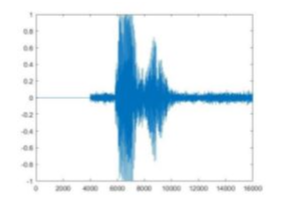
\includegraphics[width=3cm]{figures/1174008/6/teori5.PNG}
            	\centering
           	 \caption{Cara Membaca Plot MFCC}
       	 \end{figure}

        \item One-hot Encoding
One Hot Encoding mengkategorikan variabel yang mengandung nilai label dan bukan nilai numerik.

	\begin{figure}[H]
		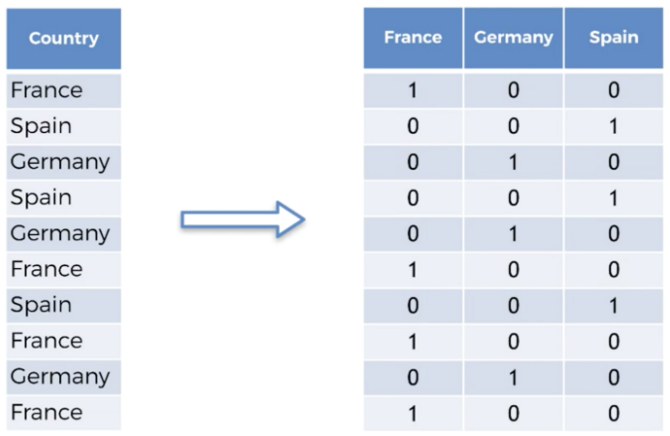
\includegraphics[width=3cm]{figures/1174008/6/teori6.PNG}
            	\centering
           	 \caption{One Hot Encoding}
       	 \end{figure}

        \item fungsi dari np.unique dan to\_categorial dalam Code Program
Kegunaan np array untuk keperluan analisis data, seperti operasi vektor dan matriks.

	\begin{figure}[H]
		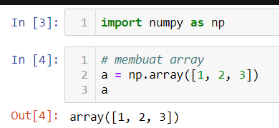
\includegraphics[width=3cm]{figures/1174008/6/teori7.PNG}
            	\centering
           	 \caption{np unique}
       	 \end{figure}

        \item fungsi dari Sequential
Pada metode sequential merupakan sebuah proses membandingkan setiap elemen atau isi sebuah larik satu per satu secara beruntun, yaitu mulai dari elemen pertama sampai dengan elemen terakhir atau elemen yang dicari sudah ditemukan.

	\begin{figure}[H]
		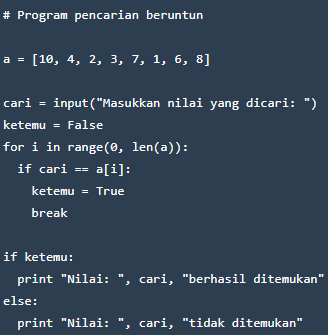
\includegraphics[width=3cm]{figures/1174008/6/teori8.PNG}
            	\centering
           	 \caption{Sequential}
       	 \end{figure}
\end{enumerate}

    \subsection{Praktek}
        \begin{enumerate}
            \item Penjelasan data GTZAN Genre Collection dan Freesound, Buat Code Program untuk Load data Tersebut.
            \subitem GTZAN Genre Collection merupakan datasets yang berisi data lagu yang terdiri dari 10 genre yaitu :
            \begin{itemize}
            \item Blues
            \item Classical
            \item Country
            \item Disco
            \item Hip-Hop
            \item Jazz
            \item Metal
            \item Pop
            \item Reggae
            \item Rock
            \end{itemize}
            10 genre tersebut memiliki data sebesar 100 data suara.
            
            \subitem sedangkan Freesound merupakan sebuah contoh suara yang digunakan untuk menguji hasil dari pengolahannya dengan menggunakan metode MFCC, untuk mencari genre yang pas bagi contoh suara tersebut.
            
            \lstinputlisting[firstline=1, lastline=10]{src/1174008/6/1174008.py}
            
            \subitem Code tersebut digunakan untuk memanggil library Librosa yang memuat metode Feature dan Display yang akan digunakan untuk memproses data suara tersebut dengan MFCC. lalu Library Glob yang digunakan untuk mencocokan pattern yang spesifik dari data tersebut, Library Numpe yang digunakan untuk membuat data Vector, Library matplotlib yang digunakan untuk membuat data grafik dan Library Keras adalah open-source yang bekerja untuk memproses TensorFlow, CNTK dan Theano, yang didesain untuk melakukan penelitian dengan menggunakan Deep Neural Network.
            
            \item Penjelasan Code Program display\_mfcc
            
            \lstinputlisting[firstline=12, lastline=22]{src/1174008/6/1174008.py}
            
            \subitem Code tersebut meliputi penggunaan MFCC dengan proses Display yang memiliki penjelasan seabgai berikut, Variable Y berisi Library Librosa dengan method LOAD dan berisi nilai SONG sebagai penggunaan classnya. dan Variable MFCC yang berisi method feature.mfcc dan memiliki nilai dari Variable Y. penggunaan plt sebagai pemanggilan matplotlib dengan method FIGURE yang akan menampilkan data gambar. dan Librosa yang akan menampilkan method display.specshow dengan data dari Variable mfcc dan pengaturan Axis X dan Y. lalu mengisikan data dengan nilai dari COLORBAR, TITLE yang berisi data dari class SONG dan tight\_layout serta show yang akan menampilkan hasil RUN yang dilakukan.
            
            \subitem dengan menggunakan code ini akan menampilkan hasil dari penggunaan display mfcc
            
            \lstinputlisting[firstline=24, lastline=25]{src/1174008/6/1174008.py}
            
            \subitem hasilnya adalah sebagai berikut, dengan menampilkan data dari file disco.00035.au dapat dilihat pada gambar
            
            \begin{figure}[H]
                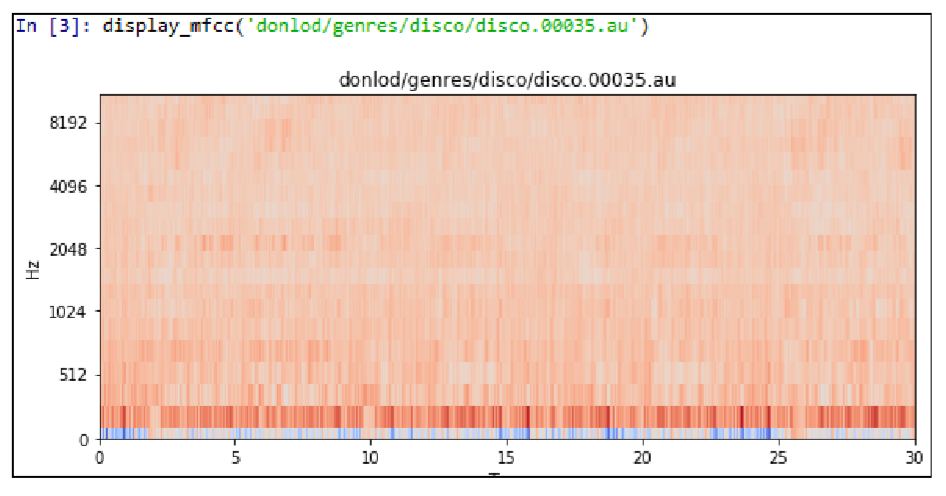
\includegraphics[width=3cm]{figures/1174008/6/1.PNG}
                \centering
                  \caption{Hasil dari Code Program display\_mfcc}
            \end{figure}
            
            \item Penjelasan Code Program extract\_feature\_song
            
            \lstinputlisting[firstline=27, lastline=36]{src/1174008/6/1174008.py}
            
            \subitem Pada Code Program diatas akan menjelaskan tentang ekstrasi data feature dari lagu yang akan di olah. dengan menggunakan Variable Y yang berisi method LOAD dengan record datanya dari class F pada extract\_feature\_song lalu membuat Variable mfcc dengan nilai yang akan meload data mfcc dari class Y, lalu melakukan normalisasi pada data Variable mfcc dengan penggunaan np.amax dengan nilai np.absolute(mfcc) lalu melakukan return dengan method np.ndarray.flatten(mfcc)[:25000] dimana data yang akan dibaca adalah sebanyak 25000 data dengan nilainya adalah array.
            
            \begin{figure}[H]
                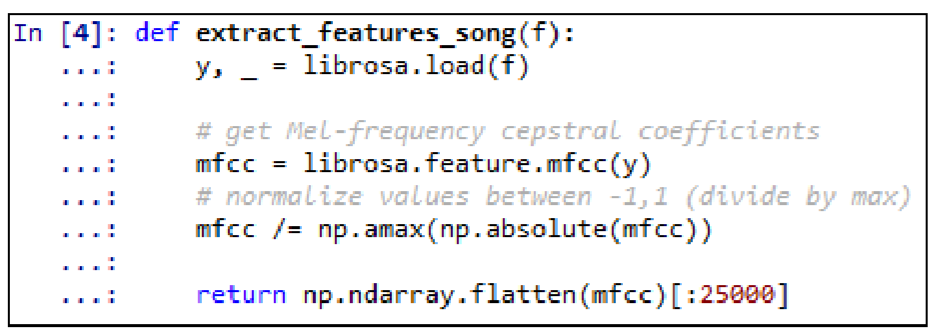
\includegraphics[width=3cm]{figures/1174008/6/2.PNG}
                \centering
                  \caption{Code Program extract\_feature\_song}
            \end{figure}
            
            
            \item Penjelasan Code program  generate\_features\_and\_labels
            
            \lstinputlisting[firstline=38, lastline=56]{src/1174008/6/1174008.py}
            
            \subitem pada code ini dimulai dengan membuat 3 data Variable array dengan format 2 nilai kosong dan 1 memiliki nilai. dimana data tersebut akan diolah dengan perintah FOR untuk membagi datasetnya sesuai dengan data GENRE yang telah ada. dengan menggunakan NUMPY pada perintah selanjutnya untuk melakukan pembagian data dan dikonversikan menjadi data one-hot encoding.
            
            \subitem hasil dari penggunaan perintah generate\_features\_and\_labels dapat dilihat pada gambar
            
            \begin{figure}[H]
                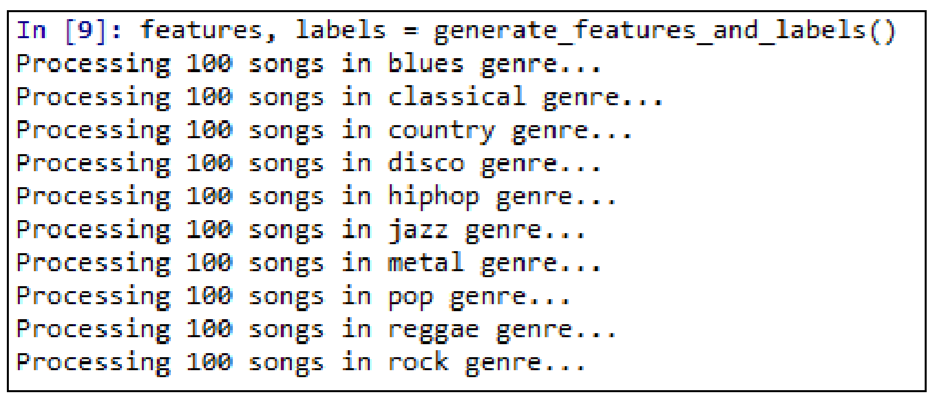
\includegraphics[width=3cm]{figures/1174008/6/3.PNG}
                \centering
                  \caption{Code Program generate\_features\_and\_labels}
            \end{figure}
            
            \item Penjelasan tentang Kenapa proses pada generate\_features\_and\_labels lama
            
            \lstinputlisting[firstline=58, lastline=59]{src/1174008/6/1174008.py}
            
            \subitem pada bagian penampilan hasil tersebut bisa lama dikarenakan data yang diolah itu tidaklah sedikit yang artinya memiliki data yang banyak, dimana masing - masing data yang diolah akan dilakukan cek terlebih dahulu untuk menentukan GENRE yang sesuai dan data tersebut akan dibagi menjadi 100 data yang telah dikonversikan menjadi data one-hot encoding.
            
            \item Penjelasan tentang pembagian data training sebesar 80 persen.
            
            \lstinputlisting[firstline=65, lastline=66]{src/1174008/6/1174008.py}
            
            \subitem pemisahan data tersebut adalah untuk memastikan bahwa sistem telah siap untuk dilakukan uji coba dengan benar, dimana sistem tersebut telah dilakukan test dengan menggunakan testing data sehingga data yang akan didapatkan nanti dari penggunaan training data tidaklah terlalu jauh untuk nilai akhirnya. hasil dari penggunaan training\_split dapat dilihat pada gambar 
            
            \begin{figure}[H]
                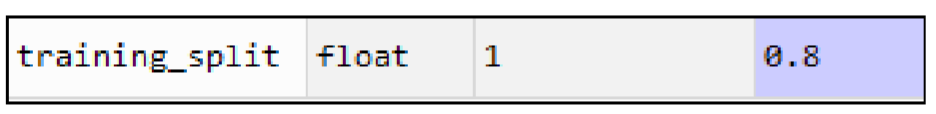
\includegraphics[width=3cm]{figures/1174008/6/4.PNG}
                \centering
                  \caption{Hasil Code Program training\_split}
            \end{figure}
            
            \subitem dan berikut ini adalah hasil akhir dari data yang telah dipisahkan menjadi data TEST dan TRAIN dengan data tersebut sudah dilakukan SHUFFLE (acak) terdapat pada gambar.
            
            \begin{figure}[H]
                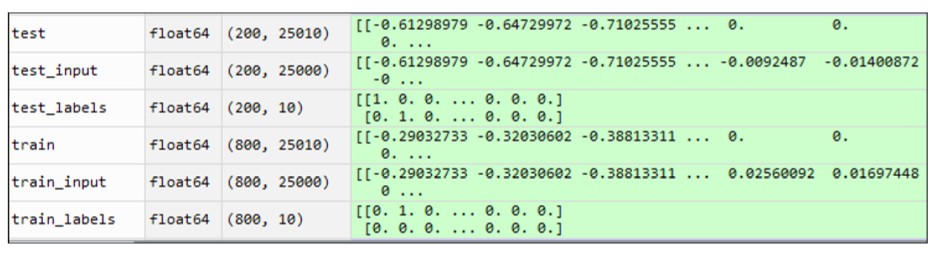
\includegraphics[width=3cm]{figures/1174008/6/5.PNG}
                \centering
                  \caption{Hasil Code Program training\_split}
            \end{figure}
            
            \item Penjelasan parameter fungsi Sequential
            
            \lstinputlisting[firstline=92, lastline=98]{src/1174008/6/1174008.py}
            
            \subitem fungsi Sequential pada code program ini adalah untuk mengolah data inputan agar sesuai dengan fungsi - fungsi yang ada pada code tersebut, dimana data yang akan diolah akan dilakukan pembentukan terlebih dahulu dengan menggunakan perintah pada Library NUMPY yaitu SHAPE dengan data yang digunakan adalah train\_input.
            
            \subitem pada gambar dibawah ini adalah keluaran dari RUNNING code tersebut
            
            \begin{figure}[H]
                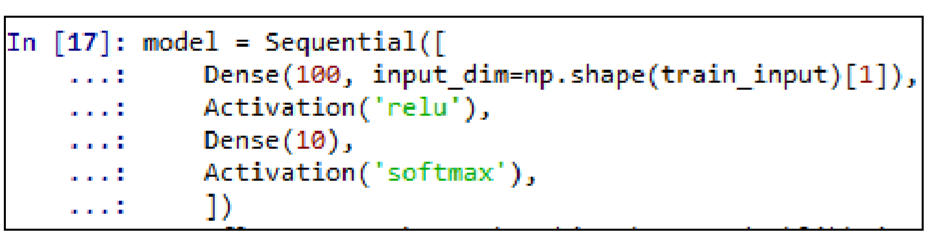
\includegraphics[width=3cm]{figures/1174008/6/6.PNG}
                \centering
                  \caption{Hasil Code fungsi Sequential}
            \end{figure}
            
            \item Penjelasan parameter fungsi Compile
            
            \lstinputlisting[firstline=100, lastline=103]{src/1174008/6/1174008.py}
            
            \subitem fungsi Compile digunakan untuk melakukan proses yang akan mengecek data parameter yang akan digunakan dari data yang telah diolah dari proses Sequential. hasil dari RUNNING pada fungsi Compile dapat dilihat pada gambar
            
            \begin{figure}[H]
                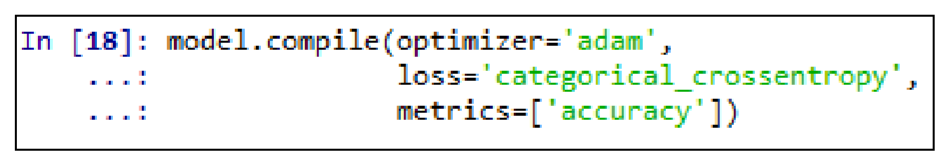
\includegraphics[width=3cm]{figures/1174008/6/7.PNG}
                \centering
                  \caption{Hasil Code fungsi Compile}
            \end{figure}
            
            \subitem pada gambar dibawah ini adalah hasil dari penjelasan tentang data Sequential dan Compile
            
            \begin{figure}[H]
                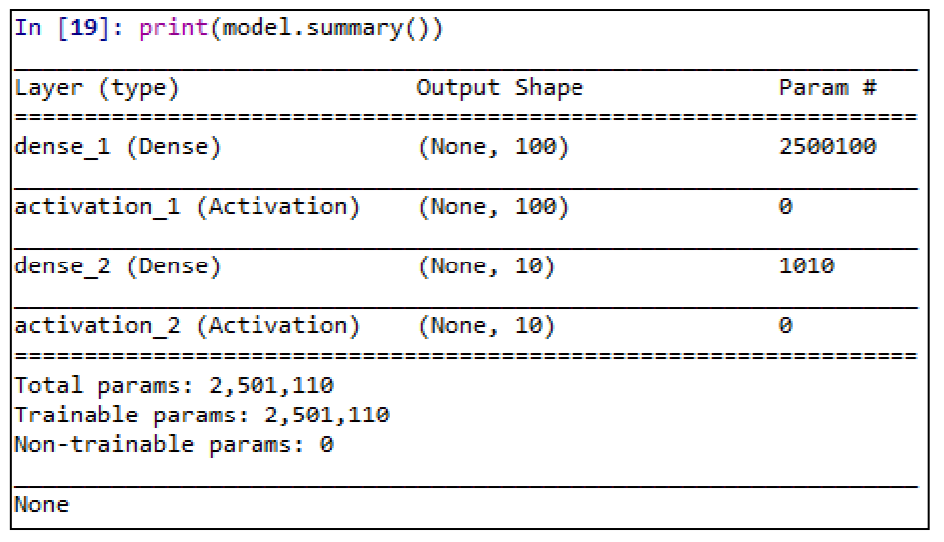
\includegraphics[width=3cm]{figures/1174008/6/8.PNG}
                \centering
                  \caption{Hasil Code Program Summary}
            \end{figure}
            
            \item Penjelasan parameter fungsi Fit
            
            \lstinputlisting[firstline=107, lastline=109]{src/1174008/6/1174008.py}
            
            \subitem fungsi Fit digunakan untuk mengolah data dari 10 label data menjadi 10 File datasets, yang kemudian akan dihitung untuk mengukur tingkat akurasi penilaiannya untuk keakuratan data yang diolah serta tingkat Loss (gagal) data yang terjadi. hasil dari RUNNING fungsi Fit dapat dilihat pada gambar.
            
            \begin{figure}[H]
                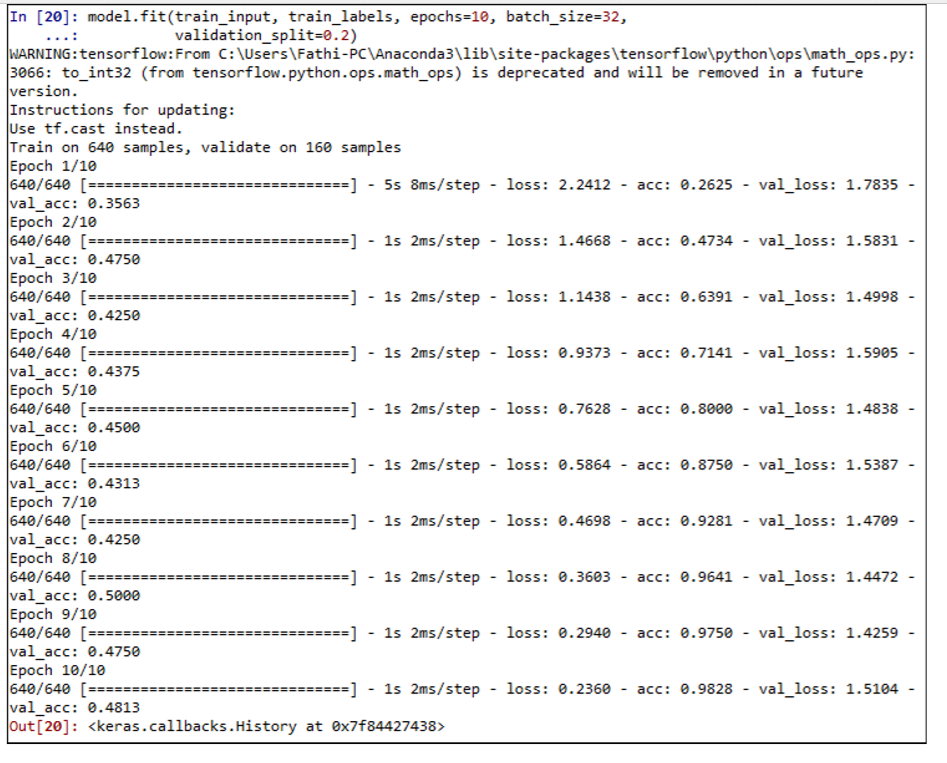
\includegraphics[width=3cm]{figures/1174008/6/9.PNG}
                \centering
                  \caption{Hasil Code fungsi Fit}
            \end{figure}
            
            \item Penjelasan parameter fungsi Evaluate
            
            \lstinputlisting[firstline=111, lastline=112]{src/1174008/6/1174008.py}
            
            \subitem fungsi Evaluate digunakan untuk mengevaluasi data yang telah diolah dengan menggunakan perintah fungsi Seqeuntial, Compile dan juga Fit. untuk hasilnya dapat dilihat pada gambar.
            
            \begin{figure}[H]
                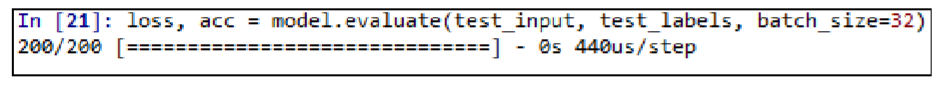
\includegraphics[width=3cm]{figures/1174008/6/10.PNG}
                \centering
                  \caption{Hasil Code fungsi Evaluate}
            \end{figure}
            
            
            \lstinputlisting[firstline=114, lastline=116]{src/1174008/6/1174008.py}
            
            \subitem untuk data yang ditampilkan pada gambar dibawah ini adalah data yang telah disusun untuk membandingkan tingkat Akurasi dan Loss yang terjadi.
            
            \begin{figure}[H]
                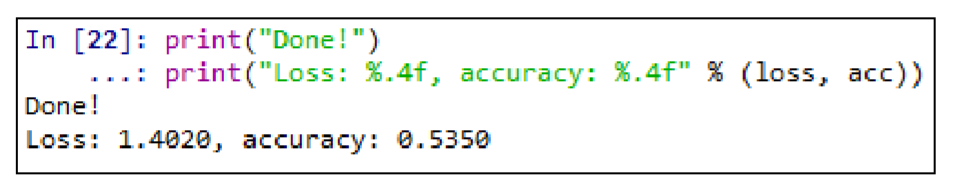
\includegraphics[width=3cm]{figures/1174008/6/11.PNG}
                \centering
                  \caption{Hasil Code fungsi Evaluate}
            \end{figure}
            
            \item Penjelasan parameter fungsi Predict
            
            \lstinputlisting[firstline=118, lastline=119]{src/1174008/6/1174008.py}
            
            \subitem fungsi Predict adalah untuk membandingkan tingkat Akurasi dari data pada setiap label yang ada pada dataset GENRE dimana data akurasi nilainya yang tertinggi maka akan diambil sebagai hasil akhir untuk nilai akurasi Predict. hasil RUNNING dapat dilihat pada gambar
            
            \begin{figure}[H]
                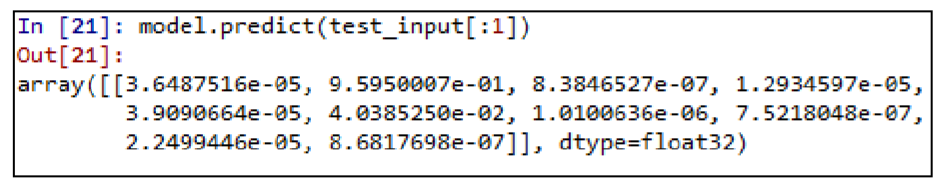
\includegraphics[width=3cm]{figures/1174008/6/12.PNG}
                \centering
                  \caption{Hasil Code fungsi Predict}
            \end{figure}
            \end{enumerate}

\subsection{Penanganan Error}

\subsection{Bukti Tidak Plagiat}
\begin{figure}[H]
\centering
	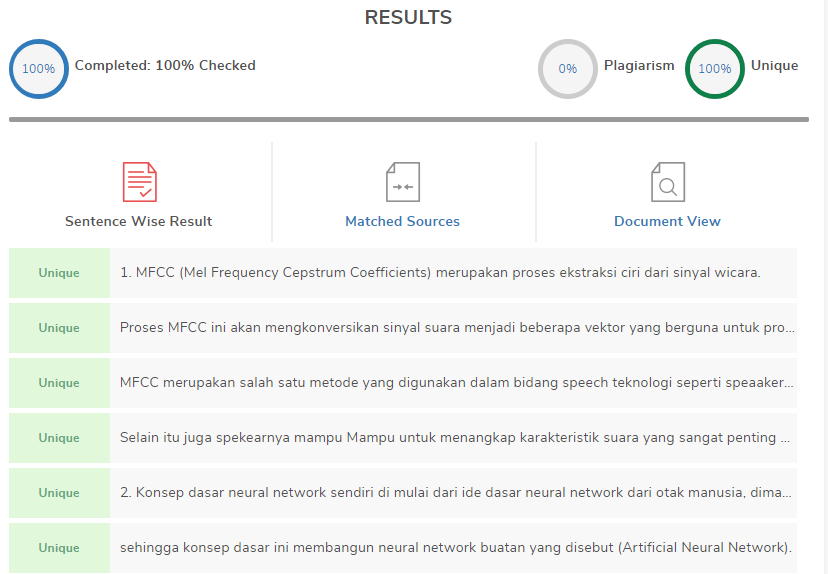
\includegraphics[width=3cm]{figures/1174008/6/bukticekplagiat.PNG}
	\caption{Bukti Tidak Melakukan Plagiat Chapter 6}
\end{figure}